\documentclass[12pt,letter]{article}


%compile with pdflatex:
%:! bibtex %:r
%:! pdflatex -synctex=1 -interaction=nonstopmode --shell-escape %

\usepackage{amsmath}
\usepackage{natbib}
\usepackage{graphicx}

\usepackage{gnuplottex}
\usepackage{booktabs}
\usepackage{subcaption}
\usepackage{caption}
\captionsetup{font={sf,small},labelfont=bf,width=0.95\textwidth}
%\usepackage{wrapfig}
\usepackage{multirow}
\newcommand{\tabitem}{~~\llap{\textbullet}~~}

\title{Bayesian analysis of lava flows:\\2012-3 Tolbachik example}
\date{May, 2015}
\author{Jacob Richardson}

\usepackage[margin=1in]{geometry}
%\usepackage{setspace}
%\doublespacing

\usepackage{titlesec}
\titleformat*{\section}{\large\bfseries} %LARGE, Large, large
\titleformat*{\subsection}{\normalsize\bfseries} %LARGE, Large, large

\usepackage{lineno}
%\linenumbers

%Geology Papers are limited to ~5000 words

\begin{document}

\maketitle

\section{Introduction}
Bayesian statistics are a primary tool by which scientists can update their belief in a certain phenomenon given new information, such as model output. Simple examples of this are often medical in nature. For instance, if a woman's female relatives have had breast cancer in their lives, she has a certain probability (i.e.~$P$(Cancer)) of having breast cancer herself. If a reliable medical test is administered and gives a positive result for breast cancer, the patient will rationally increase her belief in potentially having breast cancer, above the probability, $P$(Cancer) she assumed prior to the test. This belief updating occurs as long as the test is reliable, even if the test is not perfect. Likewise, if the test gave a negative result for cancer, she would rationally decrease her belief in having breast cancer, below $P$(Cancer).

In hazard analysis, this tool can be similarly used to test the reliability of lava flow models. Toward this, I examine the different ways that Bayesian analysis can test the capability of related lava flow spreading algorithms in forecasting the areal extent of the 2012-3 Tolbachik lava flow in Kamchakta Russia. First, I will give an outline of this eruption in Section \ref{sec:tolb_back} and a basic background on Bayesian statistics in Section \ref{sec:bayes_back}. Then I will test results from the MOLASSES lava flow model with varying ``Pulse Volume'' parameters using Bayesian statistics in Section \ref{sec:lava_app}. I will further explore the applications of Bayesian statistics when dealing with model uncertainty in a Monte Carlo fashion in Section \ref{sec:lava_MC}. The following Discussion Section will look at a way to use multiple metrics to identify an optimal model, defined as a model that most reduces unexpected economic loss, and will describe best practices to avoid artificially improving model fit statistics.


\section{Tolbachik lava flow background}\label{sec:tolb_back}
The Tolbachik lava flow began in November 2012, being originally sourced from a long fissure vent south of Tolbachik Dol. Initial magma flux was estimated to be 440~m$^3$~s$^{-1}$ \citep{belousov2015overview}. The fissure vent ultimately coalesced into two main vents, seen in TanDEM-X data and the flux dropped significantly to between 100 and 200~m$^3$~s$^{-1}$. Early stages of the flow carried lava west to a maximum runout of 14.5~km and later stages beginning in January or February, carried lava east. The total emplacement volume is $\sim$0.5~cu.~km. with 0.38~cu.~km. of that being to the west. TanDEM-X data show that the modal thickness of the flow is 7.8~m, and that the overall thickness distribution is log-normal. After the flow ceased, the total emplacement area was mapped using orthophotos and TanDEM-X data where clouds were present in the images by \citet{kubanek2015lava}.

\section{Bayes theorem background}\label{sec:bayes_back}
Bayes theorem holds that, given events $A$ and $B$ (where $A$ might be a phenomenon and $B$ might be a test result), the conditional probability of $A$ given $B$ can be described as
\begin{equation}
P(A|B)=\frac{P(B|A)P(A)}{P(B)}\label{eq_bayes}
\end{equation}
In this equation:
\begin{itemize}
	\item $P(A)$ is the \textit{prior}, the general probability of the $A$ occuring.
	\item $P(B)$ is the general probability of $B$ occuring. If $B$ is a test result, this might be referred to as model information.
	\item $P(B|A)$ is the conditional probability of the occurence of $B$ given the occurence of $A$.
	\item $P(A|B)$ is the \textit{posterior} probability of $A$ occurring given the occurence of $B$.
\end{itemize}

Three related statistical measures of model fit to a phenomenon are model sensitivity, specificity, and the Jaccard similarity coefficient. \textit{Model sensitivity} is defined as the percent of the total population within $A$ that the test $B$ correctly characterizes or models, or
\begin{equation}
\mathrm{Sensitivity} = \frac{|A\cap B|}{|A|}\label{eq_sensitivity}
\end{equation}
\textit{Model specificity} on the other hand is defined as the percent of the total population where $A$ does not occur that the lack of event $B$ correctly characterizes, or 
\begin{equation}
\mathrm{Specificity} = \frac{|\neg A\cap \neg B|}{|\neg A|}
\end{equation}
The \textit{Jaccard similarity coefficient}, or Jaccard Index, is defined as the ratio of the intersecting population of $A$ and $B$ to the union of the two populations, or
\begin{equation}
\mathrm{Jaccard~Index} = \frac{|A\cap B|}{|A\cup B|}
\end{equation}

Consider that $A$ is a natural phenomenon occuring within a population $N$ and $B$ is a test to predict $A$ for elements within the population $N$. 
\begin{itemize}
\item \textit{True positives} exist where $A$ occurs in elements and $B$ correctly predicts $A$. This can also be phrased as the intersection of $A$ and $B$, or $A\cap B$.
\item \textit{True negatives} exist where $A$ does not occur and $B$ correctly predicts the absence of $A$. This can be expressed as $\neg A\cap\neg B$.
\item \textit{False positives} exist where $A$ does not occur but $B$ incorrectly predicts $A$. This is $\neg A\cap B$.
\item \textit{False negatives} exist where $A$ does occur but $B$ incorrectly predicts the absence of $A$. This is $A\cap\neg B$.
\end{itemize}

A Bayesian treatment can use the results from $B$ to update belief of $A$, using Equation \ref{eq_bayes}. The prior probability of $A$, $P(A)$, within population $N$ is given as
\begin{equation}
P(A)=\frac{|A|}{|N|}.\label{eq_PA}
\end{equation}
The model information $P(B)$ is the percent of the population where $B$ predicts $A$ (whether correctly or not), or 
\begin{equation}
P(B)=\frac{|B|}{|N|}.\label{eq_PB}
\end{equation}
The conditional probability $P(B|A)$ is the probability of $B$ predicting $A$, given $A$. This is the percentage of true positives within the population of $A$ and is equivalent to model sensitivity.

The posterior probability of $A$ given the positive outcome of $B$, or $P(A|B)$ can then be calculated by substituting terms in Equation \ref{eq_bayes} with Equations \ref{eq_sensitivity}, \ref{eq_PA}, and \ref{eq_PB}:
\begin{align}
P(A|B)&=\frac{\frac{|A\cap B|}{|A|}\frac{|A|}{|N|}}{\frac{|B|}{|N|}}~\mathrm{,~or~simplified,}\label{eq_unsimplepost}\\
&=\frac{|A\cap B|}{|B|}.\label{eq_simplepost}
\end{align}
$P(A|B)$ can therefore be thought of as the percentage of true positives within the subpopulation characterized by $B$. This posterior probability is not dependent on the size of the population $N$, nor does it quantify false negatives (where $A$ occurs even though $B$ does not predict $A$) in any way.

\section{Application to lava flow models}\label{sec:lava_app}
A primary way that hazard forecasting models have been validated in the past has been asking the question ``What percentage of the hazard phenomenon did the model correctly forecast?'' This is essentially asking for the model sensitivity. A person at risk of loss due to the hazard might instead want to know ``If the model forecasts loss for me, what is the likelihood that loss will actually occur?'' This is the posterior probability, $P(A|B)$ discussed above.

Applied to lava flows and lava flow models, the population $N$ can be considered to be locations that might possibly be inundated with lava, given an eruption. The phenomenon $A$, in this case eventual inundation by lava, occurs or does not occur for each location and $P(A)$ is the probability of inundation within $N$. The test $B$ for each element in $N$ is an algorithm which models lava inundation and $P(B)$ is the probability of the flow simulation forecasting inundation within $N$. Equation \ref{eq_bayes} can be altered to:
\begin{equation}
P(Lava|Sim)=\frac{P(Sim|Lava)P(Lava)}{P(Sim)}\label{eq_lavabayes}
\end{equation}
where $Lava$ is the real phenomenon of lava inundation and $Sim$ is the model prediction of inundation, at any given location within the assigned hazard area of interest.

Analysis performed on the 2012-3 Tolbachik flow presents an opportunity to validate lava flow models in a Bayesian framework: pre-eruptive DEMs exist at multiple spatial resolutions (e.g.~75~m SRTM and 15~m TanDEM-X), the locations of flow inundation have been mapped, and flow parameters have been estimated or measured (e.g. magma flux at the source vents, locations of source vents, flow thickness, flow volume). Lava flow models can be run using the flow parameters and pre-eruptive DEMs as input parameters, giving the subpopulation $Sim$. The mapped lava flow provides the subpopulation $Lava$. Comparing $Sim$ for different algorithms directly with $Lava$ can then quantify the valditiy of flow algorithms in a Bayesian sense.

\paragraph{Model Execution} To populate $Sim$, I have run the MOLASSES lava flow code using TanDEM-X derived parameters, listed below:
\begin{center}
	\textbf{MOLASSES Flow Parameters}\\
	\begin{tabular}{l l}
		\toprule
		Elevation Model & 15-m bistatic TanDEM-X, 11 Nov 2015\\
		Modal Thickness & 7.8~m\\
		Pulse Volumes & 16 equally separated volumes, [1755,14917] m$^3$\\
		\midrule
		Vent$_N$ Easting & 582800~m (UTM Zone 57)\\
		Vent$_N$ Northing & 6182100~m\\
		Vent$_N$ Total Volume & 4.63$\cdot10^7$~m$^3$\\
		\midrule
		Vent$_S$ Easting & 582475~m\\
		Vent$_S$ Northing & 6180700~m\\
		Vent$_S$ Total Volume & 1.737$\cdot10^8$~m$^3$\\
		\bottomrule
	\end{tabular}
\end{center}
All variables are fixed except the ``Pulse Volume'' parameter, which is the amount of lava delivered to source cells in the Cellular Automata grid of MOLASSES.

The MOLASSES algorithm used is also fixed. The algorithm spreads lava proportional to the local slope on each side of the automaton in question, but does not have parent-child relationship laws. It is 8-connected, meaning each automaton with lava may spread lava in any or all of 8 directions in a grid around it. The chosen output of MOLASSES is an x,y,z ASCII list where x and y are easting and northing in UTM and z is the flow thickness.

Model output is compared to a list of x,y locations in the Tolbachik area that have been inundated or not. This location list is stored in a raster with the same projection and extent as the elevation model used in MOLASSES. ASCII locations output by MOLASSES are also listed in the same projection within the same extent as the elevation model. This enables direct comparison between the Model information (i.e. $Sim$) and the mapped lava flow (i.e. $Lava$). True Positives, False Positives, and False Negatives are reported as cell counts (number of grid locations where $Lava$ and $Sim$ agree or not). Three examples of these simulations are mapped in Figure \ref{fig:pulse_map}.

\begin{figure}
\centering
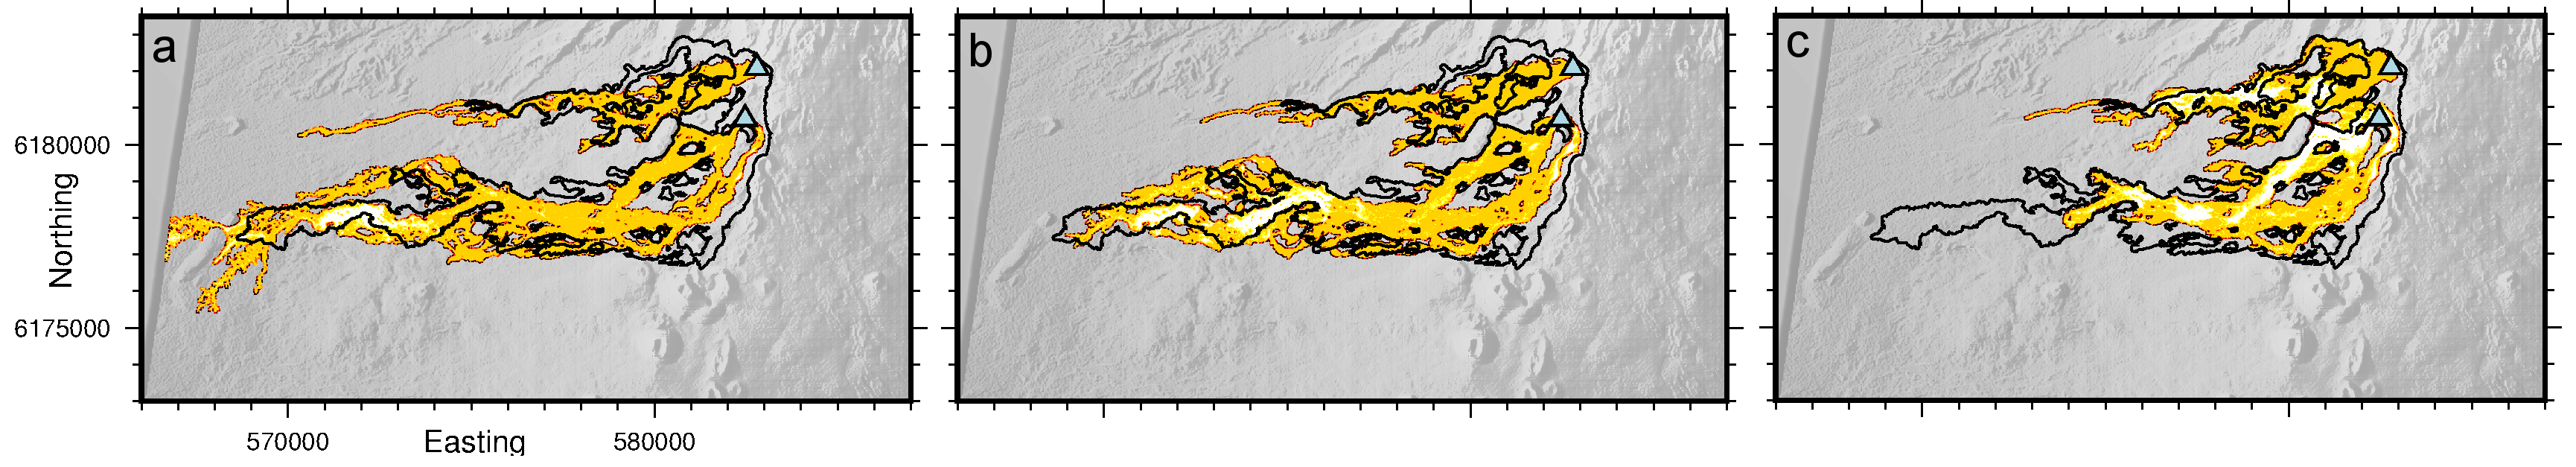
\includegraphics[width=\linewidth]{figures/3flows_h}
\caption{MOLASSES Simulations of the 2012-3 Tolbachik Lava Flows. Vents are shown as blue triangles and the mapped flow is outlined in black. a) Pulse Volume = 1755 m$^3$, the simulation far exceeds the true runout distance; b) Pulse Volume = 4387 m$^3$, this simulation performs best under the negative posterior $P(\neg Lava|\neg Sim)$ test; c) Pulse Volume = 14040 m$^3$, this simulation performs best under the posterior $P(Lava|Sim)$ test, but does not have a runout length similar to the mapped flow.}
\label{fig:pulse_map}
\end{figure}



\subsection{$P(Sim|Lava)$ (model sensitivity): Lava destroyed my home, but did the simulation predict it?}

Model sensitivity is the percentage of the true phenomenon $Lava$ that the test $Sim$ accurately predicted. A model sensitivity of 0\% would indicate that between $Lava$ and $Sim$ there were no true positives. Mathematically, the size of the union, $|Lava\cap Sim|$ is 0. A model sensitivity of 100\% would indicate that $|Lava\cap Sim|$ is the same size as $Lava$, or $|Lava\cap Sim|=|Lava|$. If model sensitivity is perfect, there are no false negatives, though there might be false positives.
\begin{figure}[h!]
	\centering
	\begin{gnuplot}[terminal=latex, terminaloptions=rotate]
		unset key
		set size 0.7, 0.7
		set format xy "$%g$"
		set xlabel "Pulse Volume" rotate by 90
		set ylabel "Sensitivity"
		set ytics 0.05
		set xtics 4000
		plot "results_bayes.dat" using 1:2 with linespoints lt 4 pt 7
	\end{gnuplot}
	\caption{Model Sensitivity for MOLASSES flows with differing Pulse Volumes.}
	\label{fig_sensitivity}
\end{figure}

\subsection{$P(Lava|Sim)$: If the simulation predicts lava inundation for a given location, what is the actual chance of lava inundation at the location?}

The posterior statistical measure is the fundamental tool of Bayesian statistics, and quantifying it enables an update of belief in risk of lava inundation. A perfect posterior value would mean that if the model simulates lava inundating a location, lava will certainly inundate that location. The posterior is calculated for simulated lava flows of different Pulse Volumes and is graphed in Figure \ref{fig_lavaGsim}. From this, it can be seen that the highest pulse volumes, which coincidentally form the shortest flow simulations, perform best with this test, with the best fit having a pulse volume of 14040~m$^3$ per algorithm loop (Figure \ref{fig:pulse_map},c). A local maximum does exist in the low pulse volumes at 4387~m$^3$ per loop.


\begin{figure}[h!]
	\centering
	\begin{gnuplot}[terminal=latex, terminaloptions=rotate]
		unset key
		set size 0.7,0.7
		set format xy "$%g$"
		set xlabel "Pulse Volume" rotate by 90
		set ylabel "$P(Lava|Sim)$"
		set ytics 0.05
		set xtics 4000
		plot "results_bayes.dat" using 1:3 with linespoints lt 4 pt 7
	\end{gnuplot}
	\caption{Posterior $P(Lava|Sim)$ for MOLASSES flows with differing Pulse Volumes.}
	\label{fig_lavaGsim}
\end{figure}

%Talk specifically about the math
%Provide examples as figures.

\paragraph{Hazard Response Implications} The higher $P(Lava|Sim)$ is for a lava spreading algorithm, the higher certainty there is that if the simulation predicts inundation, inundation will occur. Algorithms known to have high $P(Lava|Sim)$ values should influence more people to evacuate an area, if the area is predicted by those algorithms to be hit by lava. If $P(Lava|Sim)$ is low, then it is more likely that evacuating all locations simulated to be affected would be a waste of resources.

\subsection{$P(\neg Lava|\neg Sim)$: If the simulation predicts my safety, how safe am I really?}\label{sec_negpost}

The weakness of the posterior statistic explored so far ($P(Lava|Sim)$), is that it does not measure fit of the negative results of the simulation. If the simulation does not inundate a location, this posterior does not enable the ``belief of safety,'' $P(\neg Lava)$, to be updated. Therefore I propose to use a second posterior, which I will call the \textit{negative posterior}.

The negative posterior $P(\neg Lava|\neg Sim)$, or the probability of safety given simulated safety, is essentially the percentage of non-inundated area in the simulation that is also not inundated in real life. This can be found by defining this posterior using Bayes' Theorem similar to Equation \ref{eq_lavabayes}:
\begin{equation}
P(\neg Lava|\neg Sim)=\frac{P(\neg Sim|\neg Lava)P(\neg Lava)}{P(\neg Sim)}
\end{equation}
A perfect negative posterior would indicate that, if a model does not simulate a hit for a location, lava will certainly not inundate that location. While the posterior $P(Lava|Sim)$ is essentially population size blind, and does not rely on the number of true negatives (Equations \ref{eq_unsimplepost} and \ref{eq_simplepost}), this posterior does rely on true negatives. Thus, the size of the population, here referred to as the Potential Hazard Area, must be estimated \textit{a priori}.

\paragraph{Potential Hazard Area} The hazard area for the 2012-3 Tolbachik Lava Flows are simply assumed to be any location below the vent elevation plus modal flow thickness (7.8~m), within a given radius. The hazard radius is calculated from the equation given by \citet{kilburn2000lava} to predict the theoretical maximum distance, $R_{max}$ of a lava flow
\begin{equation}
R_{max}=\sqrt{\frac{3\epsilon SQ}{\rho g\kappa}}
\end{equation}
where $\epsilon$ is an empirical value related to the amount of extension of lava crust allowed before it fails (10$^{-3}$), $S$ is the tensile strength of this crust (10$^7$~Pa), $\rho$ is the lava crust density (2200~kg~m$^{-3}$), $g$ is gravitational acceleration, $\kappa$ is the bulk thermal diffusivity ($4\times 10^{-7}$~m$^{2}$~s$^{-1}$) and $Q$ is the mean volumetric flow rate from the vent. From this, the hazard radius for Tolbachik is calculated to be 39 km given a magma flux of 440~m$^3$~s from the vent as was estimated early in the eruption \citep{belousov2015overview}. The total area within this radius that is also below the vent-plus-modal-flow-thickness elevation is 1,415~km$^2$. Note that the mapped flow area of 26~km$^2$ only covers 1.9\% of this defined hazard area.

\paragraph{Results}


\begin{figure}[h!]
	\centering
	\begin{gnuplot}[terminal=latex, terminaloptions=rotate]
		unset key
		set size 0.7,0.7
		set format xy "$%g$"
		set xlabel "Pulse Volume" rotate by 90
		set ylabel "$P($not $Lava|$not $Sim)$"
		set ytics 0.001
		set xtics 4000
		plot "results_bayes.dat" using 1:4 with linespoints lt 4 pt 7
	\end{gnuplot}
	\caption{Negative posterior $P(\neg Lava|\neg Sim)$ for MOLASSES flows with differing Pulse Volumes.}
	\label{fig_neglavaGsim}
\end{figure}

The negative posteriors of simulations with different pulse values are shown in Figure \ref{fig_neglavaGsim}. Unlike the previous posterior analyzed, the best performing flows have smaller pulse volumes and the best performing volume is 4387~m$^3$ per model pulse loop (Figure \ref{fig:pulse_map},b). These results, however, show very high performance for all models, where $>$99.2\% of the area not hit by the lava flow in the potential hazard area is also not hit in all simulations. This is due to the enormous relative size of the hazard area and will be discussed later. Also of note, due to the large potential hazard area, this posterior has a very strong correlation with Model Sensitivity (Figure \ref{fig_sensitivity}). The correlation is not a coincidence. These two metrics will always have a high linear agreement given a very large abundance of true negatives. This fact is explained in an Appendix following this report.

\paragraph{Hazard Response Implications} The higher $P(\neg Lava|\neg Sim)$ is for a lava spreading algorithm, simulated safety (i.e. the similation does not predict inundation) at a given location more certainly predicts real safety at that location. This is the obverse of the previously discussed posterior metric, which relates simulated damage to actual damage. Algorithms known to have high $P(\neg Lava|\neg Sim)$ values should influence fewer people to evacuate an area that is predicted by those algorithms to be safe. If $P(\neg Lava|\neg Sim)$ is low however, it is more likely that necessary evacuations would not occur, resulting in greater loss of infrastructure or even life.

\section{Incorporating model uncertainty using Monte Carlo}\label{sec:lava_MC}
%This uses that monte carlo thing.

%Questions: What is the distribution of Bayesian statistics for all of these models?

%Bin the SIM results. If you're given an X% chance of the simulation hit, what are the bayesian statistics? (E.g. if you're given a 1-10% chance of being hit in the simulation, do you have a 1-10% chance of actually being hit?)

%Cumulatively bin the data: If you're given a >X% chance of simulation hit, what are the bayesian statistics

In this section I will explore how model uncertainty might be incorporated in model validation. Model uncertainty is a result of input parameter uncertainty, such as elevation error, and may be estimated using the Monte Carlo method for the MOLASSES code. Elevation uncertainty is added to the MOLASSES code and each model of 1,000 unique model runs is analyzed using the above statistics. The distribution of these results will first be discussed. Then different levels of simulated inundation probability will be compared to the Tolbachik flow extent.

MOLASSES flow parameters for the Monte Carlo model are listed below. 
\begin{center}
	\textbf{Monte Carlo MOLASSES Flow Parameters}\\
	\begin{tabular}{l l}
		\toprule
		Elevation Model & 75-m SRTM\\
		Elevation Uncertainty, $1\sigma$ & 3~m\\
		Residual Thickness & 7.8~m\\
		Pulse Volumes & 44200 m$^3$\\
		\midrule
		Vent$_N$ Easting & 582800~m (UTM Zone 57)\\
		Vent$_N$ Northing & 6182100~m\\
		Vent$_N$ Total Volume & 4.63$\cdot10^7$~m$^3$\\
		\midrule
		Vent$_S$ Easting & 582475~m\\
		Vent$_S$ Northing & 6180700~m\\
		Vent$_S$ Total Volume & 1.737$\cdot10^8$~m$^3$\\
		\bottomrule
	\end{tabular}
\end{center}
In this section SRTM data is used, with a spatial resolution of 75~m per pixel. Vertical uncertainty is estimated by \citet{rodriguez2006global} for Eurasia to be 6.2~m at a 90\% confidence level and is shown to be randomly distributed. Because of this, elevation uncertainty in the MOLASSES model is given a value of $1\sigma=3$~m. Each elevation value from the SRTM grid is initially assigned a value that deviates from the given elevation by a random amount with a gaussian standard deviation, $\sigma$, again set at 3~m. A lava flow is simulated over this surface. For the Monte Carlo process, this is repeated 1,000 times.

\subsection{Model fit distribution of 1,000 simulations}
The reliability of a model can be better understood by showing the distribution of model performance given model uncertainty, as opposed to treating model parameters and thus model output as completely certain. The metrics discussed above, specifically the posterior, the negative posterior, model sensitivity, and the Jaccard fit are calculated for each flow simulation based on the 2012-3 Tolbachik mapped flow. The distributions of each of these metrics is graphed in Figure \ref{fig:MC_dist}.

\begin{figure}
\centering
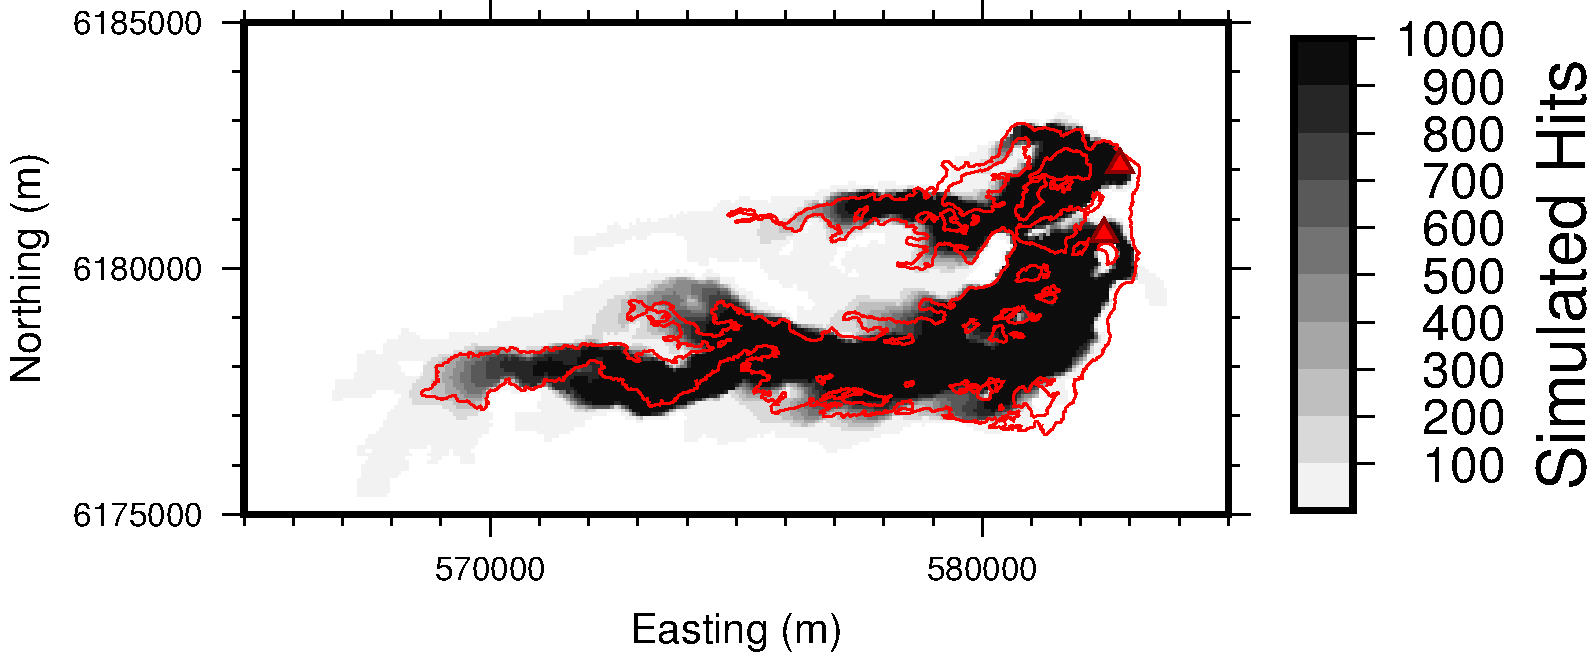
\includegraphics[width=0.7\linewidth]{figures/MC_map}
\caption{Cumulative distribution of 1,000 simulated lava flows over SRTM topography with 3~m elevation uncertainty. The red outline is the mapped flow extent of the 2012-3 Tolbachik flow. The flow source vents are mapped as red triangles.}
\label{fig:MC_map}
\end{figure}

%Graph of the performances
\begin{figure}
\centering
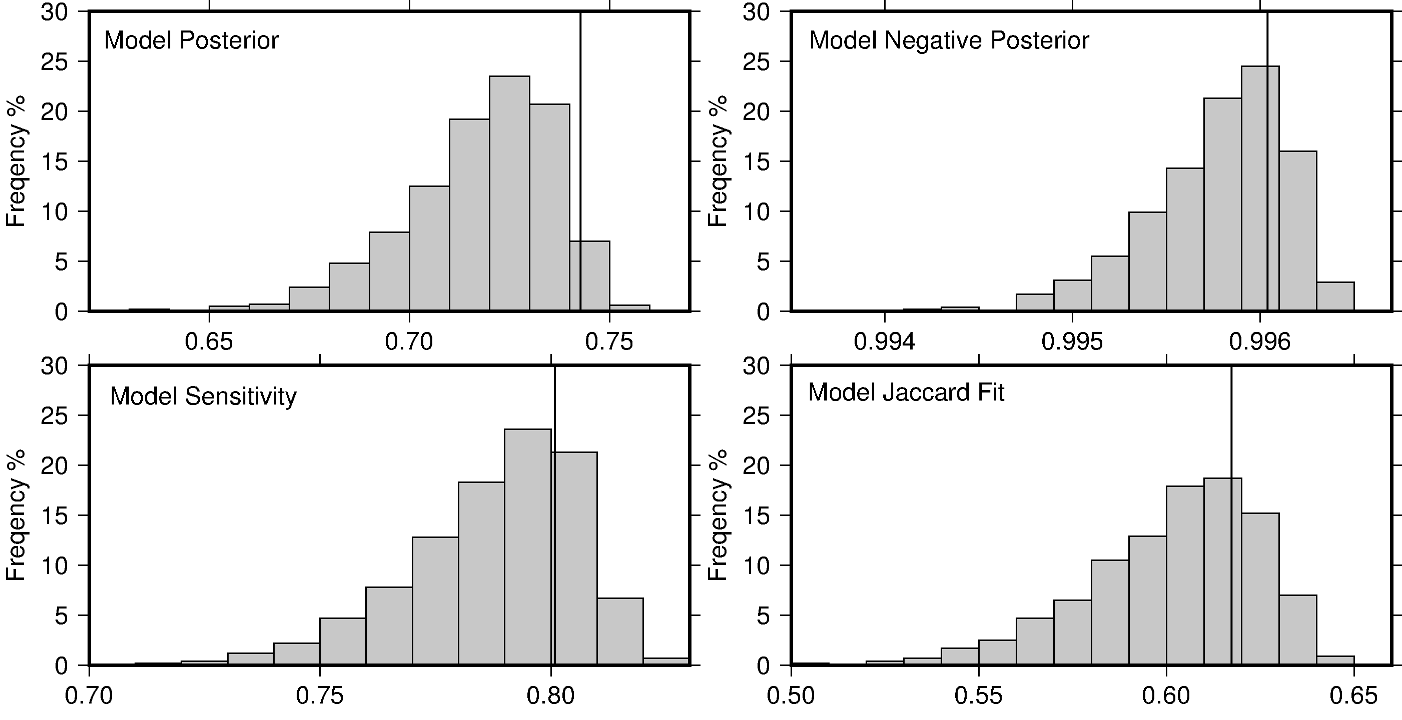
\includegraphics[width=0.7\linewidth]{figures/bayes_graphs}
\caption{Distributions of fitness statistics between the 2012-3 Tolbachik Lava Flows and 1,000 simulated lava flows over SRTM topography with 3~m standard elevation uncertainty. Vertical lines are the fitness of a simulated lava flow run over SRTM data assuming 0~m elevation uncertainty. The better than average fit for this simulation might suggest that topography is locally known better than 3~m.}
\label{fig:MC_dist}
\end{figure}


\subsection{Model fit at different simulated inundation probabilities}
By creating a cumulative map of lava flow simulations in the Monte Carlo (Figure \ref{fig:MC_map}), $P(Sim)$ may be estimated for every location as opposed to for the entire hazard area.

\begin{figure}[h!]
	\centering
	\begin{gnuplot}[terminal=latex, terminaloptions=rotate]
		unset key
		set size 0.7,0.7
		set format xy "$%g$"
		set xlabel "Minimum $P(Sim)$" rotate by 90
		set ylabel "$P(Lava|Sim)$"
		set ytics 0.1
		set ytics nomirror
		set y2tics 0.005
		set y2label "$P($not $Lava|$not $Sim)$"
		plot "results_cum.dat" using 1:6 with linespoints lt 4 pt 7 axes x1y1, "results_cum.dat" using 1:7 with linespoints lt 4 pt 6 axes x1y2, 
	\end{gnuplot}
	\caption{Bayesian Posteriors calculated for subsets of the cumulative distribution of 1,000 simulated flows in a Monte Carlo model. Black circles are posterior, $P(Lava|Sim)$ values; hollow circles are negative posterior, $P(\neg Lava|\neg Sim)$ values. Subsets are defined by all locations which have been hit by a minimum percentage of simulated flows. For instance, the far right dots are the posteriors calculated for locations inundated by every simulated flow.}
	\label{fig:MC_cum}
\end{figure}

\begin{figure}[h!]
	\centering
	\begin{gnuplot}[terminal=latex, terminaloptions=rotate]
		unset key
		set size 0.65,1
		set format xy "$%g$"
		set xlabel "$P(Sim)$" rotate by 90
		set ylabel "$P(Lava|Sim)$"
		set ytics 0.2
		set xtics 0.2
		set yrange [0:1]
		plot "results_parsed.dat" using 1:6 with points pt 7,  "results_parsed.dat" using 1:1 with lines lt 1
	\end{gnuplot}
	\caption{$P(Lava)$ calculated for locations given locations' $P(Sim)$, estimated using 1,000 simulated flows. Areas hit by 100\% of simulations are 88\% likely to be actually inundated. Areas hit by 1-5\% of simulations are about 5\% likely to be actually inundated. $P(Sim)$ is correlated with $P(Lava)$, but $P(Lava|Sim)$ rolls off at about $P(Sim)=65$\%.}
	\label{fig:MC_split}
\end{figure}

I have selected different subsets of the cumulative distribution of lava flows to evaluate using both posterior statistics, based on how many simulations hit given locations. Subsets are defined as all locations where at least a given percentage of simulated flows hit (e.g. the set of locations hit by more than 60\% of simulations, the set of locations hit by all simulations). The model fit between these subsets and the Tolbachik Flows are charted in Figure \ref{fig:MC_cum}. Points in this figure represent the probability of lava flow inundation at locations within each of these subsets. For example, 88\% of locations hit by every simulation are mapped as inundated; 75\% of locations hit by at least half of all simulations were inundated by lava; and 44\% of locations hit by at least one simulation were inundated by lava. The negative posterior is also charted in the same way: locations within the hazard area that were never hit by simulations were 99.9\% likely to remain uninundated; locations hit by fewer than half of all simulations were 99.6\% likely to not be inundated by lava; while only 98.7\% of areas remained uninundated when only locations hit by 100\% of simulations were removed.

By using this Monte Carlo method to incorporate uncertainty for an advancing lava flow, each location is assigned a probability of inundation by simulations. As the simulation is not perfect, this probability is not the same as the probability of actual inundation by lava (which is the whole reason for this report, after all). If a location is found to have a 20\% chance of inundation among simulated flows, is this similar to the probability of actual inundation? In Figure \ref{fig:MC_split} the posterior $P(Flow|Sim)$ is calculated for all locations hit by given percentages of simulations. Areas hit by $<$5\% of simulated flows all have a roughly 5\% chance of being inundated by the real flow. A positive correlation between this posterior and probability of simulation does exist in this view. The correlation appears to roll off as $P(Sim)$ approaches 65\%, as the limit of the model is reached.



\section{Discussion}\label{sec:disc}
Validation of lava flow models is important as a method of increasing the value of models to forecast lava flow processes, thereby decreasing preventable loss. Preventable loss can either be loss of property due to lava or expenditure of resources on a lava flow that never comes. Because loss of property is necessarily more valuable than a loss of resources to protect that property (since, if the resources to protect the property were more valuable, it would not make sense to use those resources), the posterior probability $P(\neg Lava|\neg Sim)$ is more important that the posterior probability $P(Lava|Sim)$. However, because $P(\neg Lava|\neg Sim)$ is dependent on the population size (i.e. the potential hazard area), it is harder to quantify.

\paragraph{Using Bayesian statistics to compare models}

In the pulse volume exercise, both the posterior and the negative posterior metrics were calculated for a number of simulations with differing pulse volumes. One pulse volume, 14040~m$^3$ per loop, performed best using the posterior statistic (Figure \ref{fig_lavaGsim}) and another, 4387~m$^3$ per loop, performed best using the negative posterior (Figure \ref{fig_neglavaGsim}). An optimal pulse volume can be identified if these metrics are given weight and compared. Because it is likely more important to have fewer false negatives (where destruction is unexpected) than false positives (where evacuation occurs but is not eventually needed), one might weight the negative posterior more importantly than the other posterior.

To score simulations by combining the posteriors, I have normalized both posteriors so the worst scoring flow has a value of 0 and the best has a score of 1. I then took a weighted average of the normalized posteriors assuming the negative posterior is 10, 5, 2, and 1 times as important as the other posterior. These are graphed on the right of Figure \ref{fig:jaccard_combined}. Luckily, regardless of the weighting, the same pulse volume is always ranked highest (4387~m$^3$ per loop).

It is interesting to note that the Jaccard Fit for these simulations (plotted on the left side of Figure \ref{fig:jaccard_combined}) is similar in shape to the weighted scores. The Jaccard fit is most similar to the combined scores where the posterior and negative posterior are given equal weight. In this case the correlation between the combined scores and the Jaccard fits have an r$^2$ value of 0.98.

%%%%NOTES%%%%
%The Jaccard model appears to be related to both posterior functions
%Changing Population size (Improvement in neg Post and Improvement in learning)
%Weighted average


\begin{figure}
\centering
\begin{subfigure}{.5\textwidth}
  \centering
	\begin{gnuplot}[terminal=latex, terminaloptions=rotate]
		unset key
		set size 0.6,0.7
		set format xy "$%g$"
		set xlabel "Pulse Volume" rotate by 90
		set ylabel "Jaccard Fit"
		set ytics 0.02
		set xtics 5000
		plot "results_bayes.dat" using 1:5 with linespoints lt 4 pt 7
	\end{gnuplot}
  \label{fig:sub1}
\end{subfigure}%
\begin{subfigure}{.5\textwidth}
  \centering
	\begin{gnuplot}[terminal=latex, terminaloptions=rotate]
		unset key
		set size 0.6,0.7
		set format xy "$%g$"
		set xlabel "Pulse Volume" rotate by 90
		set ylabel "Combined Score"
		set ytics 0.1
		set xtics 5000
		plot "results_combinedpost.dat" using 1:7 with linespoints lt 4 pt 1, "results_combinedpost.dat" using 1:5 with linespoints lt 4 pt 7, "results_combinedpost.dat" using 1:6 with linespoints lt 4 pt 3, "results_combinedpost.dat" using 1:4 with linespoints lt 4 pt 6,
		
	\end{gnuplot}
  \label{fig:sub2}
\end{subfigure}
\caption{Left, Jaccard Fit for MOLASSES flows with differing Pulse Volumes. Right, model score based on weighted averages between the posterior metric and the negative posterior metric. Hollow circles, negative posterior is 10 times weight of posterior; solid circles, 5 times weight; asterisks, 2 times weight; plusses, equal weight between posteriors.}
\label{fig:jaccard_combined}
\end{figure}

\subsection{Falsely improving value metrics}

It is possible to game the value metrics (i.e. model sensitivity and both posteriors), making a model appear better than it actually is at replicating the true flow, though steps can be taken to avoid this. Model sensitivity can be increased by increasing true positives regardless of false positives. The posterior $P(Lava|Sim)$ can be increased by reducing false positives regardless of false negatives. The posterior $P(\neg Lava|\neg Sim)$ can be decreased by artificially reducing the potential hazard area or increased by artificially increasing this area. Examples are given below.

\paragraph{Gaming examples}
As a flow simulation increases in areal extent, its model sensitivity will not decrease as long as inundated locations remain inundated. Because of this, a large flow that covers the entire hazard area will have a perfect model sensitivity score as it correctly predicts destruction of lava everywhere where lava actually will result. This hypothetical model however has little to no value in actually forecasting lava flow inundation. Again, model sensitivity can be gamed by increasing true positives without concern for false positives. 

The posterior $P(Lava|Sim)$ can also be increased at the expense of actual model value. If the lava simulation extent covers a very small area centered, perhaps, at the lava source vents, the lava simulation will be less likely to have false positives. By reducing false positives, closer to 100\% of the simulation will actually be inundated by lava, increasing $P(Lava|Sim)$.

As the posterior $P(\neg Lava|\neg Sim)$ is dependent on the hazard area size, changing this size can make this value better or worse for a model. By increasing the potential hazard area, the ``safe''-simulated area agrees more with the true ``safe'' area, as the true negatives increase proportional to false negatives. However, the usefulness of the model with increased hazard area decreases simply because $P(Lava)$ also decreases dramatically. If a house, for instance, is 100~km away and uphill from an erupting volcanic vent, $P(\neg Lava|\neg Sim)$ at the house's address does not impact the belief of its owners as $P(\neg Lava)$ is already almost certain. Also, after a certain hazard area size, it appears that models can be accurately compared against each other independent of hazard area size.

Decreasing hazard area size however can make the  $P(\neg Lava|\neg Sim)$ of certain models worse artificially. As the hazard area approaches the area of the union between the lava flow and the simulation, true negatives are removed from the population. As $P(\neg Lava|\neg Sim)$ relies on only true negatives and false negatives, false negatives gain a higher proportion in this situation. If the hazard area is defined as the model and flow union area, the only model negative locations will be false negatives, and $P(\neg Lava|\neg Sim)$ will be 0. A model with 1 false negative in this situation will be worse than a model with 0 false negatives and hundreds of false positives.

\paragraph{Avoiding value metric gaming} Several steps can be taken to insure the above metrics are useful in analyzing the value of lava flow models. First and foremost, the flow simulation results should replicate reality in more ways than areal extent. Specifically, simulation volume and ultimate flow thickness should be similar to the actual lava flow or potential flow. Constraining and checking these two values post-simulation will constrain the simulated areal extent to be similar to the actual lava flow. This secures the validity of model sensitivity and the posterior $P(Lava|Sim)$. 

Second, the hazard area should be defined based on geographic and geologic information, which essentially creates a more simple lava flow model (possibly ``Type II'' from \citet{harris2013lava}) that encompasses all possible lava-affected areas (i.e. it has a near 100\% model sensitivity and a low specificity on purpose). In Section \ref{sec_negpost} for instance, I follow Kilburn's maximum runout distance equation and assign the hazard area to be anywhere below the vent within the maximum distance in any direction. This however gives very high $P(\neg Lava|\neg Sim)$ values, $P(Lava)$ is small for the entire area, so a better hazard area might be defined some other way. One possibility is by identifying catchments that the lava flow could possibly enter \citep{kauahikaua1995applications} and using the maximum distance method on those smaller areas.



\section{Conclusions}
Regardless of how a lava flow model is chosen, its value in forecasting lava flow hazards can be quantified using Bayesian statistics. Whether the model is bad or good, if it can be compared against a real life lava flow such as the 2012-3 Tolbachik flow, the two posteriors discussed in this paper can be calculated.

By calculating $P(\neg Lava|\neg Sim)$, one may update their belief of safety based on a negative, or not-hit, result from the simulation. By calculating $P(Lava|Sim)$, one may update their belief of destruction by lava based on a positive hit result from the simulation. These two tools are potentially the most important metrics by which decision makers should base their faith in a given lava flow model.

By comparing the posterior values of multiple lava flow algorithms, the best lava flow algorithm can be identified. The more important posterior metric is the $P(\neg Lava|\neg Sim)$, as a low value would indicate more false negatives, resulting in more unpredicted destruction. $P(Lava|Sim)$ is important but less so as low values indicate more false positives, which results in greater levels of unpredicted non-destruction. While these are a trade off, selecting the best model to decrease economic loss can be achieved by taking a weighted average of the two statistics. The weight given to each would depend on potential social or economic loss from evacuation or destruction of property. In this report, the best Pulse Volume was identified to be 4387~m$^3$ over TanDEM-X data in this area.

The two Bayesian posteriors are an improvement over model sensitivity and specificity as they provide a probability estimate that a simulated result is correct. By incorporating model uncertainty and performing a Monte Carlo for the MOLASSES lava flow algorithm, $P(Sim)$ can be estimated for each given location, improving the usefulness of Bayesian statistics in hazard analysis.


\bibliographystyle{abbrvnat}
\bibliography{lava_bayes}

\section*{Appendix: Correlation between negative posterior, $P(\neg Lava|\neg Sim)$, and model sensitivity, $P(Sim|Lava)$, in large hazard areas}
\paragraph{Claim:} Given a lava flow, $Lava$, and a simulation, $Sim$, in a hazard area, $N$, it can be stated that
\begin{equation}
P(\neg Lava|\neg Sim) < aP(Sim|Lava)+b
\label{eqap_neglin}
\end{equation}
where $a=P(Lava)$ and $b= P(\neg Lava)$. Furthermore, as the area $N$ is expanded, $P(\neg Lava|\neg Sim)$ approaches a linear relationship with model sensitivity so that
\begin{equation}
P(\neg Lava|\neg Sim)\approx aP(Sim|Lava)+b
\end{equation}
Regardless of the size of $N$, $P(\neg Lava|\neg Sim)$ is never larger than the left side of this equation.

\paragraph{Proof:} Consider the table below, which divides $N$ into four quadrants, all of which have non-negative sizes.
\begin{center}
\begin{tabular}{ r | c | c |}
	\multicolumn{1}{l}{}&\multicolumn{1}{p{3em}}{\centering$Lava$} &\multicolumn{1}{p{3em}}{$\neg Lava$}\\ \cline{2-3}
	$Sim$ & $w$ & $x$ \\ \cline{2-3}
	$\neg Sim$ & $y$ & $z$ \\ \cline{2-3}
\end{tabular}
\end{center}
Quadrant $w$ represents true positives; $x$, false positives; $y$, false negatives; and $z$, true negatives. The size of $N$ is equivalent to $w+x+y+z$ and the size of $Lava$ is $w+y$. Using this notation, Priors and model sensitivity can be rewritten as:
\begin{align}
P(Lava) &= \frac{w+y}{w+x+y+z}\label{eqap_plava}\\
P(\neg Lava) &= \frac{x+z}{w+x+y+z}\\
P(Sim|Lava) &= \frac{w}{w+y}
\end{align}
The posterior $P(\neg Lava|\neg Sim)$ is given as:
\begin{equation}
P(\neg Lava|\neg Sim)=\frac{z}{y+z}
\label{eqap_postneglava}
\end{equation}
Rewriting Equation \ref{eqap_neglin} with Equations \ref{eqap_plava}-\ref{eqap_postneglava}, we can show the relationship more clearly.
\begin{align}
\frac{z}{y+z}&<\left(\frac{w+y}{w+x+y+z}\right)\left(\frac{w}{w+y}\right)+\frac{x+z}{w+x+y+z}\\
&<\frac{w}{w+x+y+z}+\frac{x+z}{w+x+y+z}\nonumber\\
&<\frac{w+x+z}{w+x+y+z}\nonumber
\end{align}
The formula $w+x$ is equivalent to the simulation size, $|Sim|$, giving
\begin{equation}
\frac{z}{y+z}<\frac{|Sim|+z}{|Sim|+y+z}
\label{eqap_qed}
\end{equation}
which is true. In the scenario where flow and simulation size are fixed, both sides of Equation \ref{eqap_qed} are also proportional. By increasing the size of $N$ with a constant flow and simulation size, only $z$ increases. If $z\gg|Sim|$, the left side (equivalent to $P(\neg Lava|\neg Sim)$, Eq. \ref{eqap_postneglava}) approaches the right. \textbf{Therefore in large hazard areas, the posterior $P(\neg Lava|\neg Sim)$ is strongly correlated to model sensitivity, $P(Sim|Lava)$.}


%\begin{figure}
%\centering
%\includegraphics[width=\linewidth]{map_diff}
%\label{fig:map_diff}
%\end{figure}


\end{document}
